\documentclass[border=4pt]{standalone}
\usepackage{amsmath,amssymb,tikz}
\usetikzlibrary{arrows.meta}
\definecolor{figB}{RGB}{31,90,166}\definecolor{figR}{RGB}{176,48,48}\definecolor{figG}{RGB}{46,125,50}
\begin{document}
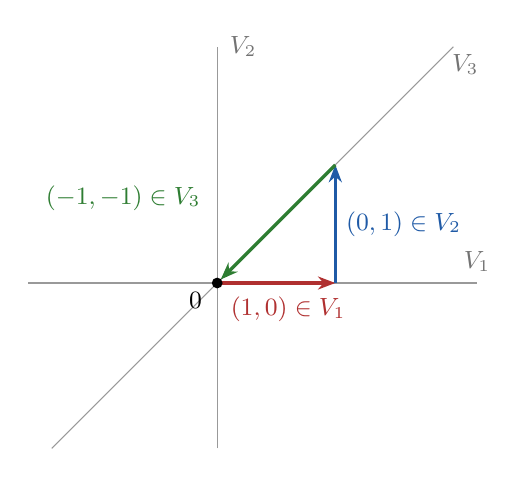
\begin{tikzpicture}[scale=1.5,>={Stealth[length=2.2mm]}]
\draw[black!40,thin] (-1.6,0)--(2.2,0); \draw[black!40,thin] (0,-1.4)--(0,2.0); \draw[black!40,thin] (-1.4,-1.4)--(2.0,2.0);
\node[black!55,font=\small] at (2.2,0.18) {$V_1$};
\node[black!55,font=\small] at (0.22,2.0) {$V_2$};
\node[black!55,font=\small] at (2.1,1.85) {$V_3$};
\draw[->,very thick,figR] (0,0)--(1,0) node[pos=0.6,below,font=\small,yshift=-1pt]{$(1,0)\in V_1$};
\draw[->,very thick,figB] (1,0)--(1,1) node[midway,right,font=\small]{$(0,1)\in V_2$};
\draw[->,very thick,figG] (1,1)--(0.03,0.03) ;
\node[figG,font=\small,anchor=east] at (-0.06,0.72) {$(-1,-1)\in V_3$};
\fill (0,0) circle(1.3pt) node[below left,font=\small,xshift=-2pt]{$0$};
\end{tikzpicture}
\end{document}
